% --------------------------------------------------
% 
% This chapter is for HPC
% 
% --------------------------------------------------

\chapter{
   0s and 1s in marine molecular research: a regional HPC perspective
}
\label{cha:hpc}


\textbf{Citation:}
Zafeiropoulos, H., Gioti, A., Ninidakis, S., Potirakis, A., Paragkamian, S., ... \& 
Pafilis, E. (2021). 0s and 1s in marine molecular research: a regional HPC perspective. 
GigaScience, 10(8), giab053, doi: \href{https://doi.org/10.1093/gigascience/giab053}{10.1093/gigascience/giab053}\footnote{
   For author contributions, please refer to the relevant section. Modified version of the published review.
}


% ZORBA ABSTRACT
   \section{Abstract}
   High-performance computing (HPC) systems have become indispensable for modern marine research, 
   providing support to an increasing number and diversity of users. Pairing with the impetus 
   offered by high-throughput methods to key areas such as non-model organism studies, their 
   operation continuously evolves to meet the corresponding computational challenges. 

   Here, we present a Tier 2 (regional) HPC facility, operating for over a decade at the 
   Institute of Marine Biology, Biotechnology, and Aquaculture of the Hellenic Centre for Marine Research in Greece. 
   Strategic choices made in design and upgrades aimed to strike a balance between depth 
   (the need for a few high-memory nodes) and breadth (a number of slimmer nodes), as dictated by the 
   idiosyncrasy of the supported research. 
   Qualitative computational requirement analysis of the latter revealed the diversity of marine fields, 
   methods, and approaches adopted to translate data into knowledge. 
   In addition, hardware and software architectures, usage statistics, policy, and user management aspects 
   of the facility are presented. Drawing upon the last decade's experience from the different levels of operation 
   of the Institute of Marine Biology, Biotechnology, and Aquaculture HPC facility, a number of lessons are presented; 
   these have contributed to the facility's future directions in light of emerging distribution technologies (e.g., containers) 
   and Research Infrastructure evolution. 
   In combination with detailed knowledge of the facility usage and its upcoming upgrade, 
   future collaborations in marine research and beyond are envisioned.


   % ZORBA INTRODUCTION
   \section{Introduction}

   The ubiquitous marine environments (more than 70\% of the global surface \citep{noaa}) 
   mold Earth's conditions to a great extent. 
   The interconnected abiotic \citep{falkowski2008microbial} and biotic factors 
   (from bacteria \citep{falkowski2008microbial} to megafauna \citep{estes2016megafaunal}), 
   shape biogeochemical cycles \citep{arrigo2005marine} and climates \citep{boero2007conceptual, beal2011role} 
   from local to global scales. 
   In addition, marine systems have high socio-economic value \citep{remoundou2009valuation} 
   as an essential source of food and by supporting renewable energy and transport, 
   among other services \citep{portner2019ocean}. 
   The study of marine environments involves a series of disciplines (scientific fields): 
   from Biodiversity \citep{sala2006global} and Oceanography to (eco)systems biology \citep{tonon2015marine} 
   and from Biotechnology \citep{dionisi2012bioprospection} to Aquaculture \citep{tidwell2001fish}.

   To shed light on the evolutionary history of (commercially important) 
   marine species \citep{carvalho1995molecular}, as well as on how invasive species respond and 
   adapt to novel environments \citep{sakai2001population}, 
   the analysis of their genetic stock structure is fundamental \citep{begg1999holistic}. 
   Similarly, biodiversity assessment is essential to elucidate ecosystem functioning \citep{loreau2000biodiversity} 
   and to identify taxa with potential for bioprospecting applications \citep{leal2012trends}. 
   Furthermore, systems biology approaches provide both theoretical and technical backgrounds 
   in which integrative analyses flourish \citep{norberg2001phenotypic}. 
   However, conventional methods do not offer the information needed to explore the 
   aforementioned scientific topics.
   
   High-throughput sequencing (HTS) and sister methods have launched a new era in many 
   biological disciplines \citep{mardis2008next, kulski2016next}. 
   These technologies allowed access to the genetic, transcript, protein, and metabolite 
   repertoire \citep{goodwin2016coming} of studied taxa or populations, and facilitated the analysis of 
   organism-environment interactions in communities and ecosystems \citep{bundy2009environmental}. 
   Whole-genome sequencing and whole-transcriptome sequencing approaches provide valuable 
   information for the study of non-model taxa \citep{cahais2012reference}. 
   This information can be further enriched by genotyping-by-sequencing approaches, 
   such as restriction site-associated DNA sequencing \citep{baird2008rapid}, or by investigating gene 
   expression dynamics through Differential Expression (DE) analyses \citep{tarazona2011differential}. 
   Moving from single species to assemblages, molecular-based identification and functional 
   profiling of communities has become available through marker (metabarcoding), 
   genome (metagenomics), or transcriptome (metatranscriptomics) sequencing from environmental 
   samples \citep{goldford2018emergent}. 
   To a great extent, these methods address the problem of how to produce and get access 
   to the information on different biological systems and molecules.

   These $0$s and $1$s of information (i.e., the data) come along with challenges regarding their 
   management, analysis, and integration \citep{merelli2014managing}. 
   The computational requirements for these tasks exceed the capacity of a standard laptop/desktop by far, 
   owing to the sheer volume of the data and to the computational complexity of the bioinformatic algorithms 
   employed for their analysis. 
   For example, building the de novo genome assembly of a non-model Eukaryote may require algorithms 
   of nondeterministic polynomial time complexity. 
   This analysis can reach up to several hundreds or thousands of GB of memory (RAM) \citep{sohn2018present}. 
   Hence, the challenges of how to exploit all these data and how to transform data into knowledge set 
   the present framework in biological research \citep{greene2014big, pal2020big}.
   
   To address these computational challenges, the use of high-performance computing (HPC) systems 
   has become essential in life sciences and systems biology \citep{lampa2013lessons}. 
   HPC is the scientific field that aims at the optimal incorporation of technology, methodology, 
   and the application thereof to achieve “the greatest computing capability possible at any point 
   in time and technology" \citep{sterling2017high}. 
   Such systems range from a small number to several thousands of interconnected computers (compute nodes). 
   According to the Partnership for Advanced Computing in Europe, the European HPC facilities are categorized as: 
   (i) European Centres (Tier 0), 
   (ii) national centers (Tier 1), and 
   (iii) regional centers (Tier 2) [33] \citep{enwiki:1009652575}. 
   As the Partnership for Advanced Computing in Europe highlights, "computing drives science and science drives computing" 
   in a great range of scientific fields, from the endeavor to maintain a sustainable Earth to efforts to expand 
   the frontiers in our understanding of the universe \citep{lindahl2018scientific}. 
   On top of the heavy computational requirements, biological analyses come with a series of other practical issues 
   that often affect the bioinformatics-oriented HPC systems.

   Researchers with purely biological backgrounds often lack the coding skills or even the 
   familiarity required for working with Command Line Interfaces \citep{lindahl2018scientific}. 
   Virtual Research Environments are web-based e-service platforms that are particularly useful 
   for researchers lacking expertise and/or computing resources \citep{candela2013virtual}. 
   Another common issue is that most analyses include a great number of steps, with the software 
   used in each of these having equally numerous dependencies. A lack of continuous support 
   for tools with different dependencies, as well as frequent and non-periodical versioning of the latter, 
   often results in broken links and further compromises the reproducibility of analyses [36]. 
   Widely used containerization technologies—e.g., Docker \citep{rad2017introduction} and Singularity \citep{kurtzer2017singularity}—ensure reproducibility 
   of software and replication of the analysis, thus partially addressing these challenges. 
   By encapsulating software code along with all its corresponding dependencies in such containers, 
   software packages become reproducible in any operating system in an easy-to-download-and-install 
   fashion, on any infrastructure.

   % ZORBA CONTRIBUTION
   \section{Contribution}

   The \href{https://imbbc.hcmr.gr/}{Institute of Marine Biology Biotechnology and Aqua-culture (IMBBC)} 
   has been developing a computing hub that, in conjunction with national and European Research Infrastructures (RIs), 
   can support state-of-the-art marine research. 
   The regional IMBBC HPC facility allows processing of data that derive from the Institute's sequencing platforms 
   and expeditions and from multiple external sources in the context of interdisciplinary studies. 
   Here, we present insights from a thorough analysis of the research supported by the facility and some 
   of its latest usage statistics in terms of resource requirements, computational methods, and data types; 
   the above have contributed in shaping the facility along its lifespan.


   % ZORBA METHODS
   \section{Methods}

   \subsection{The IMBBC HPC Facility: From a Single Server to a Tier 2 System}

   The IMBBC HPC facility was launched in 2009 to support computational needs over a range of scientific 
   fields in marine biology, with a focus on non-model taxa [39]. 
   The facility was initiated as an infrastructure of the Institute of Marine Biology and Genetics of 
   the Hellenic Centre for Marine Research.
   Its development has followed the development of national RIs (Fig. 1; 
   also see Section A1 in Zafeiropoulos et al. \citep{haris_zafeiropoulos_2021_4665308}). 
   The first nodes were used to support the analysis of data sets generated from methods such as eDNA metabarcoding and multiple omics. 
   Since 2015, the facility also supports Virtual Research Environments, including e-services and virtual laboratories. 
   The current configuration of the facility presented herein is named \textit{Zorba} (Fig. 1, Box 4) and will be upgraded within 2021 (see Section Future Directions). 
   Hereafter, \textit{Zorba} refers to the specific system setup from 2015 and onwards, while the facility throughout its lifespan will be referred to as "IMBBC HPC".

   \begin{figure}
      \centering
      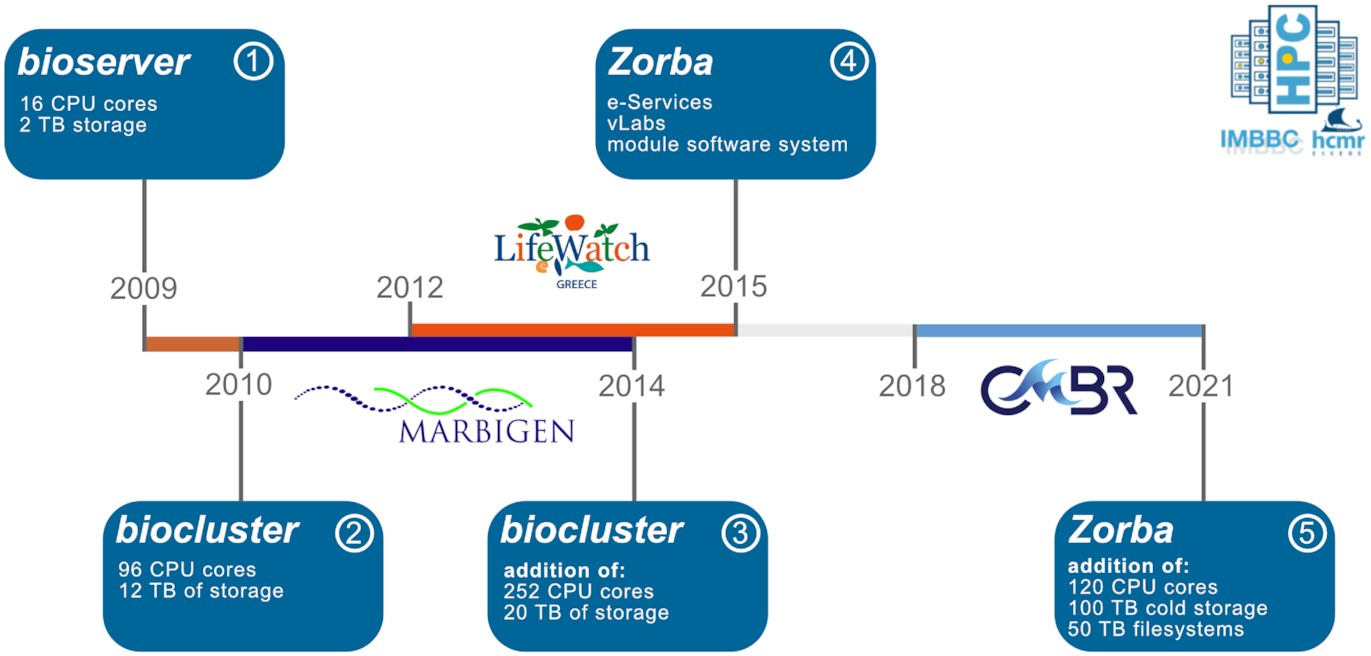
\includegraphics[width=85mm]{figures/imbbc_hpc_facility.jpeg}
      \caption[The IMBBC HPC facility history]{
         Evolution of the IMBBC HPC facility during the past 12 years, with hardware upgrades (blue boxes) and funding milestones (logos of RIs) highlighted. 
         A single server that launched the bioinformatics era in 2009 evolved to the current Tier 2 system Zorba (Box 4), which allows processing of a wide variety of information from DNA sequences to biodiversity data. 
         Different names of the facility denote distinct system architectures.
      }
   \end{figure}



   \textit{Zorba} currently consists of 328 CPU cores, 2.3 TB total memory, and 105 TB storage. 
   Job submission takes place on the 4 available computing partitions, or queues, as explained in Fig. 2. \textit{Zorba} at its current state achieves a peak performance of 8.3 trillion double-precision floating-point operations per second, or 8.3 Tflops, as estimated by LinPack benchmarking \citep{dongarra2003linpack}. 
   On top of these, a total 7.5 TB is distributed to all servers for the storage of environment and system files. 
   Interconnection of both the compute and login nodes takes place via an infiniband interface with a capacity of 40 Gbps, which features very high throughput and very low latency. 
   Infiniband is also used for a switched interconnection between the servers and the 4 available file systems. 
   A thorough technical description of \textit{Zorba} is available in Section A2 of Zafeiropoulos et al.  \citep{haris_zafeiropoulos_2021_4665308}.


   \begin{figure}
      \centering
      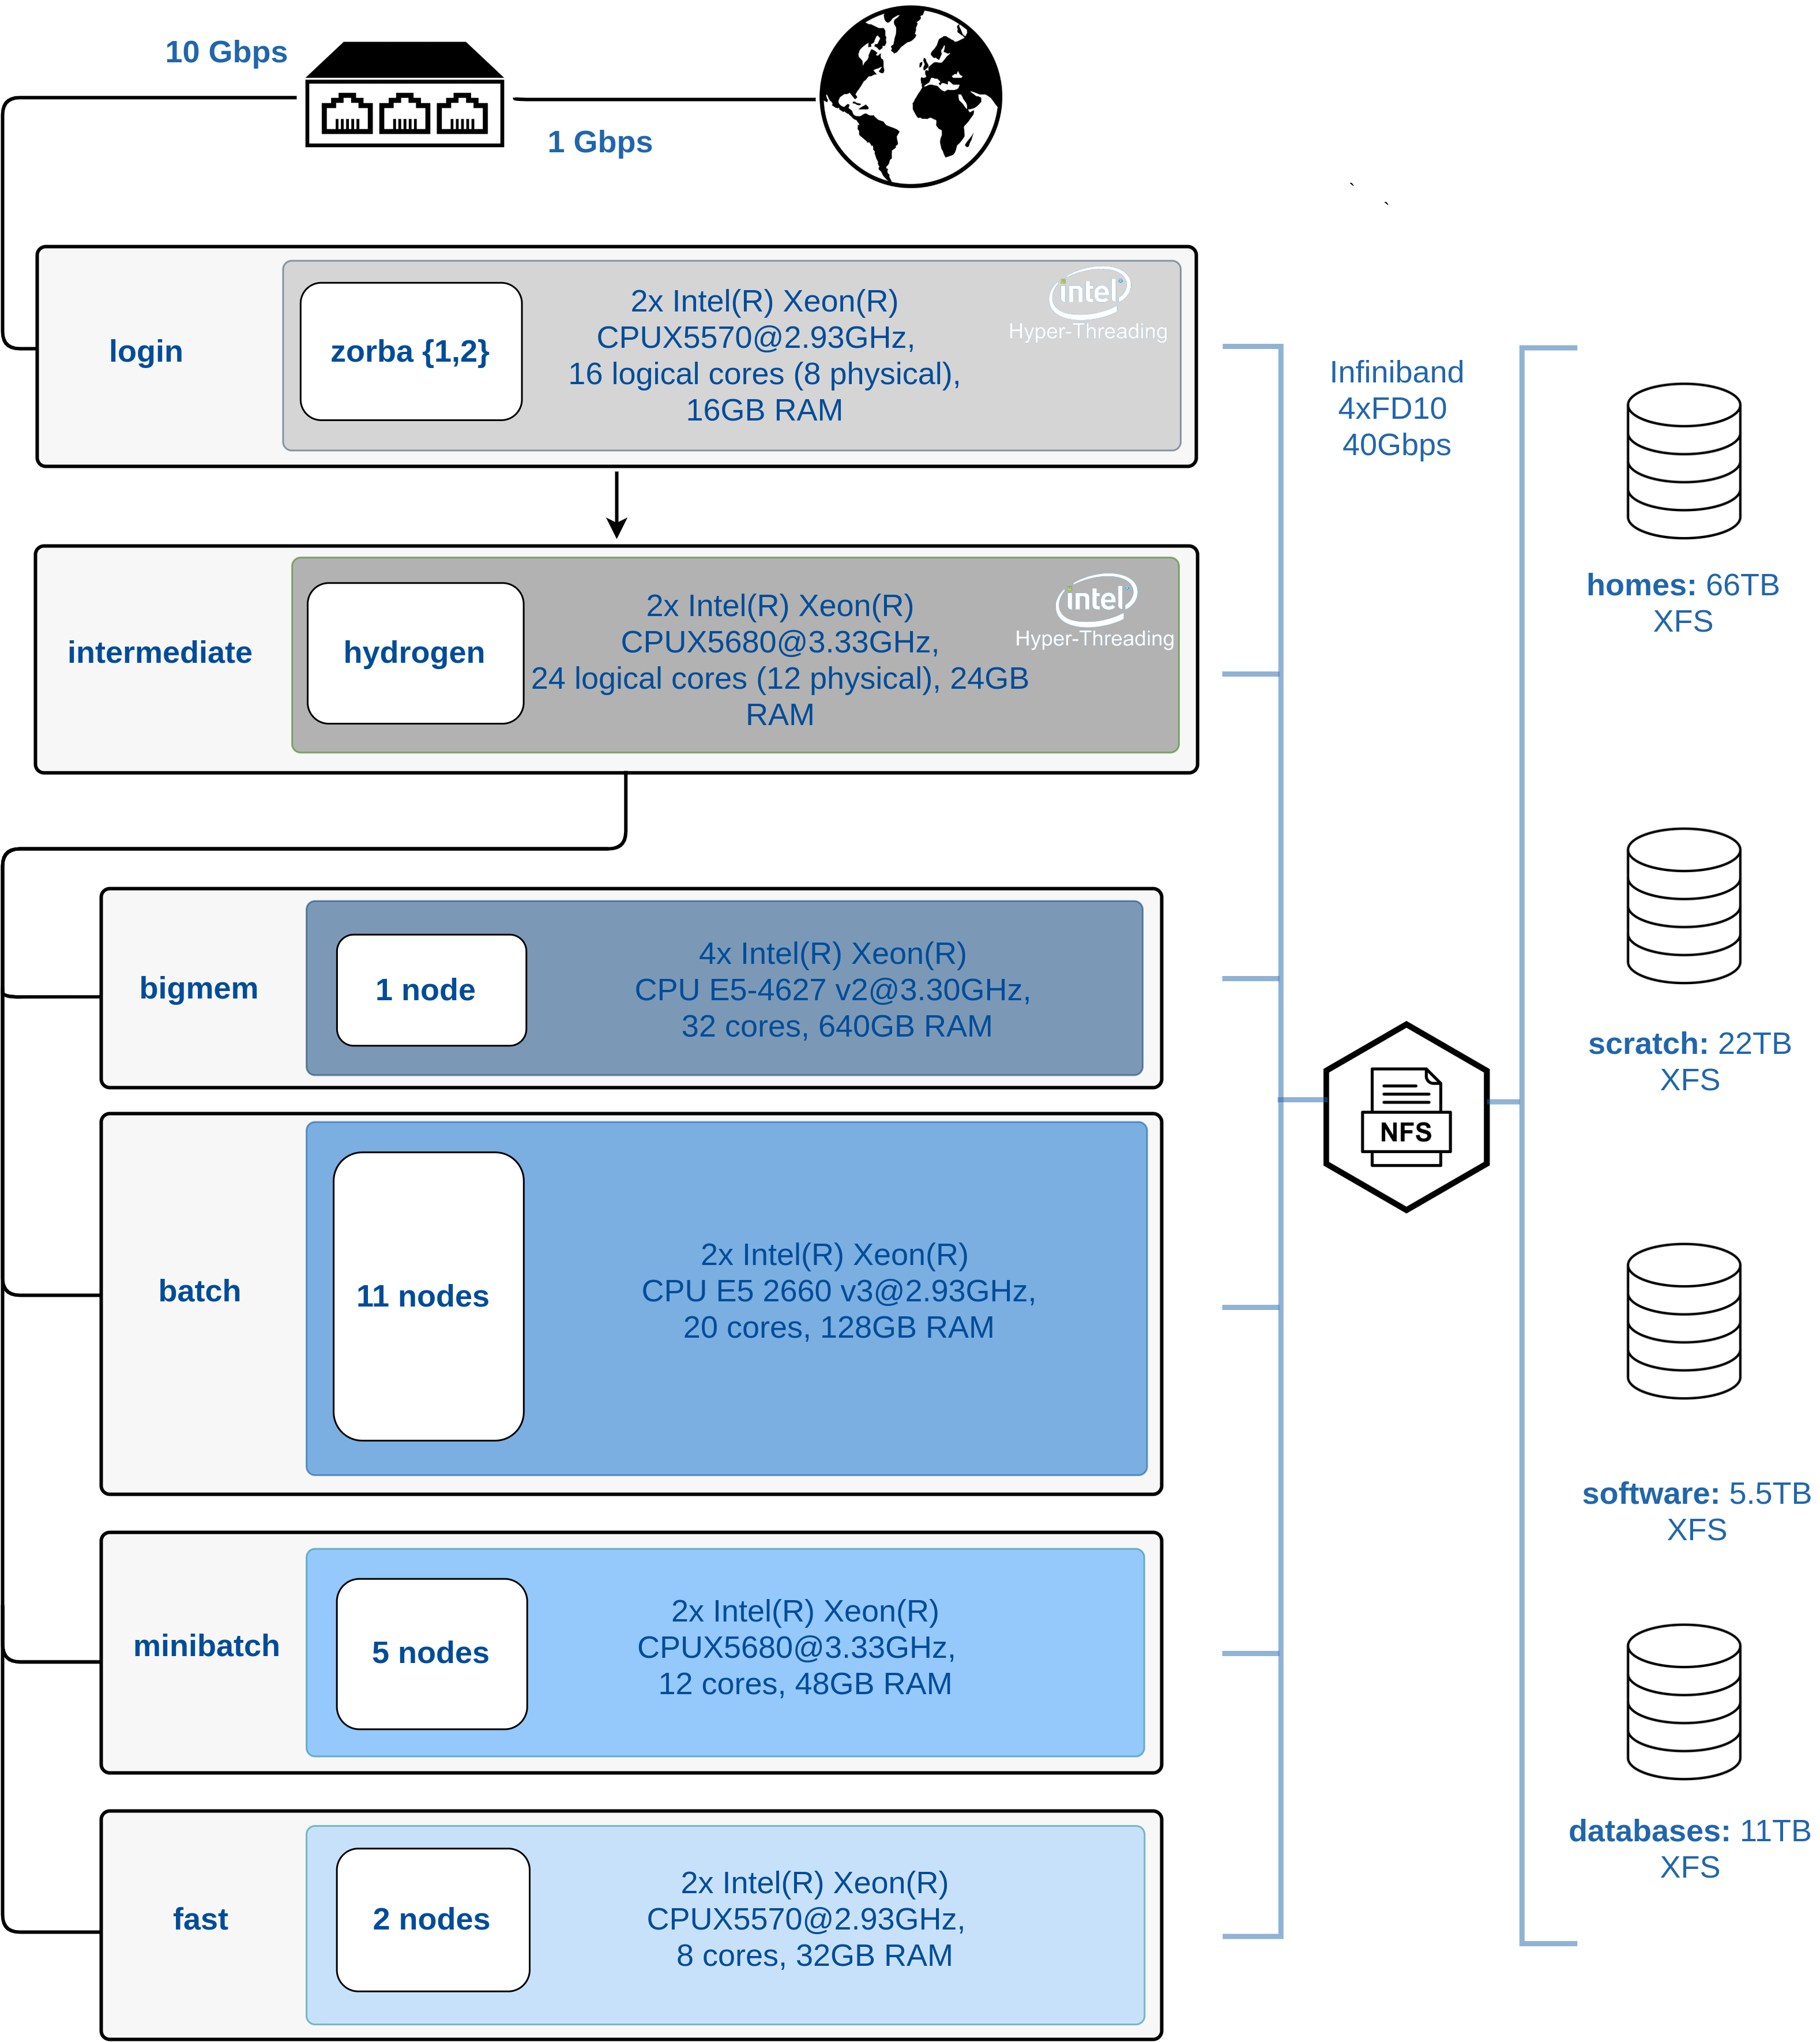
\includegraphics[width=\columnwidth]{figures/zorba_architecture.png}
      \caption[Block diagram of the \textit{Zorba} architecture.]{
         Block diagram of the \textit{Zorba} architecture.
         This is the IMBBC HPC facility architecture in its current setup, after 12 years of development. 
         There are 2 login nodes and 1 intermediate where users may develop their analyses. 
         Computational nodes are split into 4 partitions with different specs and policy terms: 
         \texttt{bigmem} supporting processes requiring up to 640 GB RAM, batch handling mostly 
         (but not exclusively) parallel-driven jobs (either in a single node or across several nodes), 
         \texttt{minibatch} aiming to serve parallel jobs with reduced resource requirements, and \texttt{fast} partition for non-intensive jobs. 
         All servers, except file systems, run Debian 9 (kernel 4.9.0-8-amd64). 
         CCBY icons from the Noun Project: "nfs file document icon" by IYIKON, PK; "Earth" 
         By mungang kim, KR; "database": By Vectorstall, PK; "switch" by Bonegolem, IT
      }
   \end{figure}





   More than \href{https://hpc.hcmr.gr/software/}{200 software packages} are currently installed and available to users at \textit{Zorba}, covering the most common analysis types. 
   These tools allow assembly, HTS data preprocessing, phylogenetic tree construction, ortholog finding, and population structure modeling, to name a few. 
   Access to these packages is provided through \href{https://modules.readthedocs.io/en/latest/index.html}{Environment Modules}, a broadly used means of accessing software in HPC systems \citep{castrignano2020elixir}.

   During the last 2 years, \textit{Zorba} has been moving from system-dependent pipelines previously developed at IMBBC (e.g., \href{https://github.com/jacqueslagnel/ParaMetabarCoding}{ParaMetabarCoding}) towards containerization of available and new pipelines/tools.
   A complete metabarcoding analysis tool for various marker genes (PEMA) \citep{zafeiropoulos2020pema}, the chained and automated use of STACKS, software for population genetics analysis from short-length sequences \citep{catchen2013stacks} (\href{https://nellieangelova.github.io/RADseq_Containers/}{latest version}), a set of statistical functions in R for the computation of biodiversity indices, and analyses in cases of high computational demands \citep{varsos2016optimized}, as well as a programming workflow for the automation of biodiversity historical data curation (\href{https://github.com/lab42open-team/deco}{DECO}) are among the in-house developed containers. 
   The standard container/image format used on \textit{Zorba} is Singularity. 
   Singularity images can be served by any \textit{Zorba} partition; 
   Docker images can run instantly as Singularity images. 
   A thorough description of the software containers developed in \textit{Zorba} can be found in Section D of Zafeiropoulos et al. \citep{haris_zafeiropoulos_2021_4665308}.

   \textit{Zorba}'s daily functioning is ensured by a core team of 4 full-time, experienced staff: a hardware officer, 2 system administrators, and a permanent researcher in biodiversity informatics and data science.

   More than 70 users (internal and external scientists), investigators, postdoctoral researchers, technicians, and doctoral/postgraduate students have gained access to the HPC infrastructure thus far.
   Support is provided officially through a help desk ticketing system. 
   An average of 31 requests/month have been received (since June 2019), with the most demanded categories being troubleshooting (38.2\%) and software installation (23.8\%). 
   Since October 2017, monthly meetings among HPC users have been established to regularly discuss such issues.

   Proper scheduling of the submitted jobs and fair resource sharing is a major task that needs to be confronted day to day. 
   To address this, a specific \href{https://hpc.hcmr.gr/docs/getting-started/policy/}{usage policy} for each of the various partitions and a scheduling software tool set have been adopted in \textit{Zorba}. 
   Policy terms are dynamically adapted to the HPC hardware architecture and to the usage statistics, with revisions being discussed between the HPC core team and users. 
   The Simple Linux Utility for Resource Management (SLURM) open-source cluster management system orchestrates the job scheduling and allocates resources, and a \href{https://booking-hpc.hcmr.gr/day.php}{booking system} helps users to organize their projects and administrators to monitor the resource reservations on a mid- to long-term basis. 
   A SLURM Database Daemon (slurmdbd) has also been installed to allow logging and recording of job usage statistics into a separate SQL database (see Section C1 in Zafeiropoulos et al.  \citep{haris_zafeiropoulos_2021_4665308}). 
   An extended description of user and job administrations and orchestration can be found in Section C1 of Zafeiropoulos et al. \citep{haris_zafeiropoulos_2021_4665308}).

   Training has been an integral component of the HPC facility mindset since its launch and enables knowledge sharing across MSc and PhD students and researchers within and outside the Institute. 
   Introductory courses are organized on a regular basis, aimed at familiarizing new users with Unix environments, programming, and HPC usage policy and resource allocation (e.g., job submission in SLURM).
   Furthermore, the IMBBC HPC facility has served, since 2011, as an international training platform for specific types of bioinformatic analyses (see Section C2 in Zafeiropoulos et al. \citep{haris_zafeiropoulos_2021_4665308}). 
   For instance, the facility has provided computational resources for workshops on 
   \href{http://www.marbigen.org/content/microbial-diversity-genomics-and-metagenomics}{Microbial Diversity, Genomics and Metagenomics}, 
   \href{http://www.marbigen.org/content/workshop-genomics-biodiversity}{Genomics in Biodiversity},
   \href{https://sites.google.com/site/workshopimbg/}{Next-Generation Sequencing technologies and informatics tools for studying marine biodiversity and adaptation in the long term}, or
   \href{https://summer-schools.aegean.gr/EcoDAR2014}{Ecological Data Analysis using R}. 
   The plan is to enhance and diversify the educational component of the HPC facility by providing courses on a more permanent basis and targeting a larger audience. 
   An extensive listing of training activities is given in Section C2 of Zafeiropoulos et al. \citep{haris_zafeiropoulos_2021_4665308}.


   % ZORBA RESULTS
   \section{Results}

   \subsection{Computational Breakdown of the IMBBC HPC-Supported Research}

   Systematic labelling of IMBBC HPC-supported published studies ($n = 47$) was performed to highlight their resource requirements. 
   Each study was manually labelled with the relevant scientific field, the data acquisition method, the computational methods, and its resource requirements; 
   all the annotations were validated by the corresponding authors (see Section D2 in Zafeiropoulos et al. \citep{haris_zafeiropoulos_2021_4665308}). 
   It should be stated that the conclusions of this overview are specific to the studies conducted at IMBBC.

   The scientific fields of Aquaculture ($~40\%$ of studies), Biodiversity ($~26\%$ of studies), and Organismal biology ($~19\%$ of studies) account for the majority of the research publications supported by the IMBBC HPC facility (Fig. 3; Supplementary File \\
   \texttt{imbbc\_hpc\_labelling\_data.xlsx} in Zafeiropoulos et al. \citep{haris_zafeiropoulos_2021_4665308}).
   

   \begin{figure}
      \centering
      \label{fig:studies}
      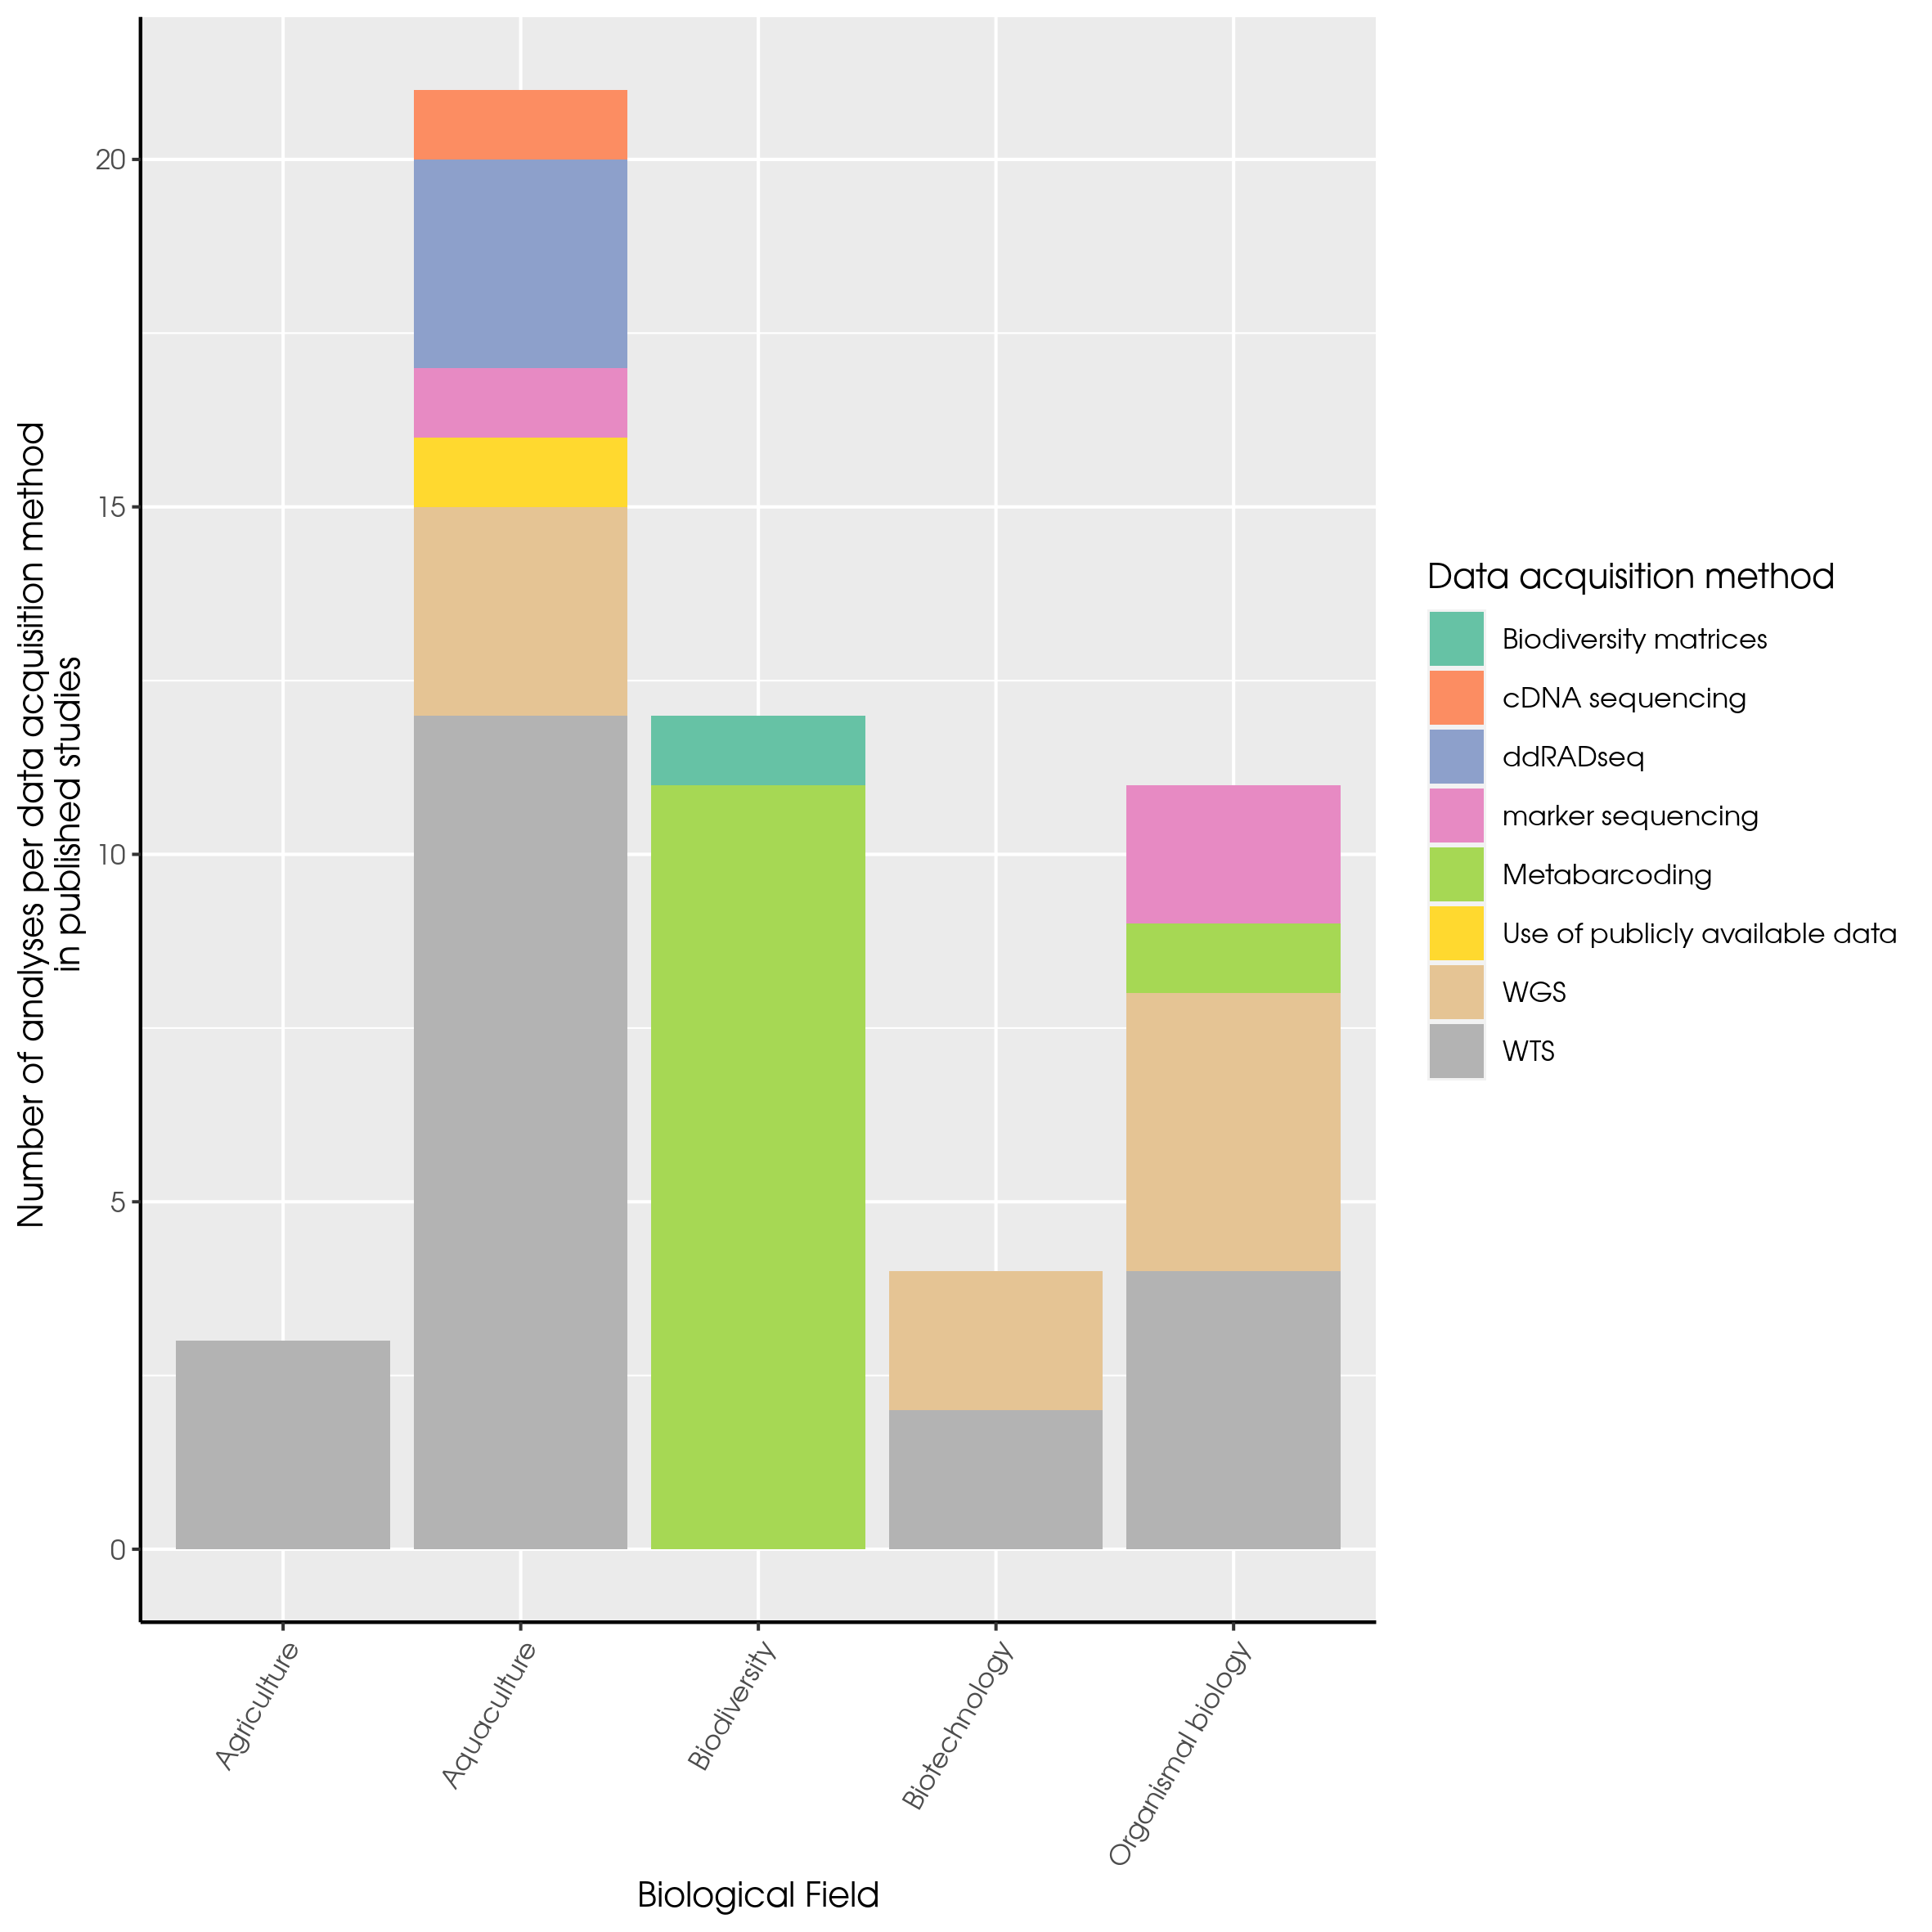
\includegraphics[width=0.6\textwidth]{figures/number_of_studies_biological_field_data_acquisition_method_plot.png}
      \caption[IMBBC HPC supported published studies grouped by scientific field]{
         Bar chart with the number of publications that have used IMBBC HPC facility resources, grouped by scientific field. The different methods for data acquisition are also presented. WGS, whole-genome sequencing; WTS, whole-transcriptome sequencing.
      }

   \end{figure}


   In comparison, studies in the Biotechnology and Agriculture fields indicate contemporary and beyond-marine orientations of research at IMBBC, respectively (see Section B2 in Zafeiropoulos et al. [40]). 
   In addition, $8$ methods of data acquisition (experimental or \textit{in silico}) have been defined (Fig. 3). 
   Among these methods, whole-genome sequencing and whole-transcriptome sequencing have been widely used in multiple fields (Biotechnology, Organismal Biology, Aquaculture). 
   Conversely, Double digest restriction-site associated sequencing (ddRADseq) has been solely employed for population genetic studies in the context of Aquaculture.

   The $47$ published studies employed different computational methods (sets of tasks executed on the HPC facility). 
   These studies served different purposes, from a range of bioinformatics analyses to HPC-oriented software optimization. 
   The computational methods were categorized in $8$ classes (Fig. 4). 
   The resource requirements of each computational method were evaluated in terms of memory usage, computational time, and storage. Reflecting the current \textit{Zorba} capacity, studies which, in any part of their analysis, exceeded $128$ GB of memory or/and $48$ hours of running time or/and $200$ GB physical space were classified as studies with high demands (see Supplementary file \texttt{imbbc\_hpc\_labelling\_data.xlsx} in \citep{haris_zafeiropoulos_2021_4665308}).


   \begin{figure}
      \label{fig:resource}
      \centering
      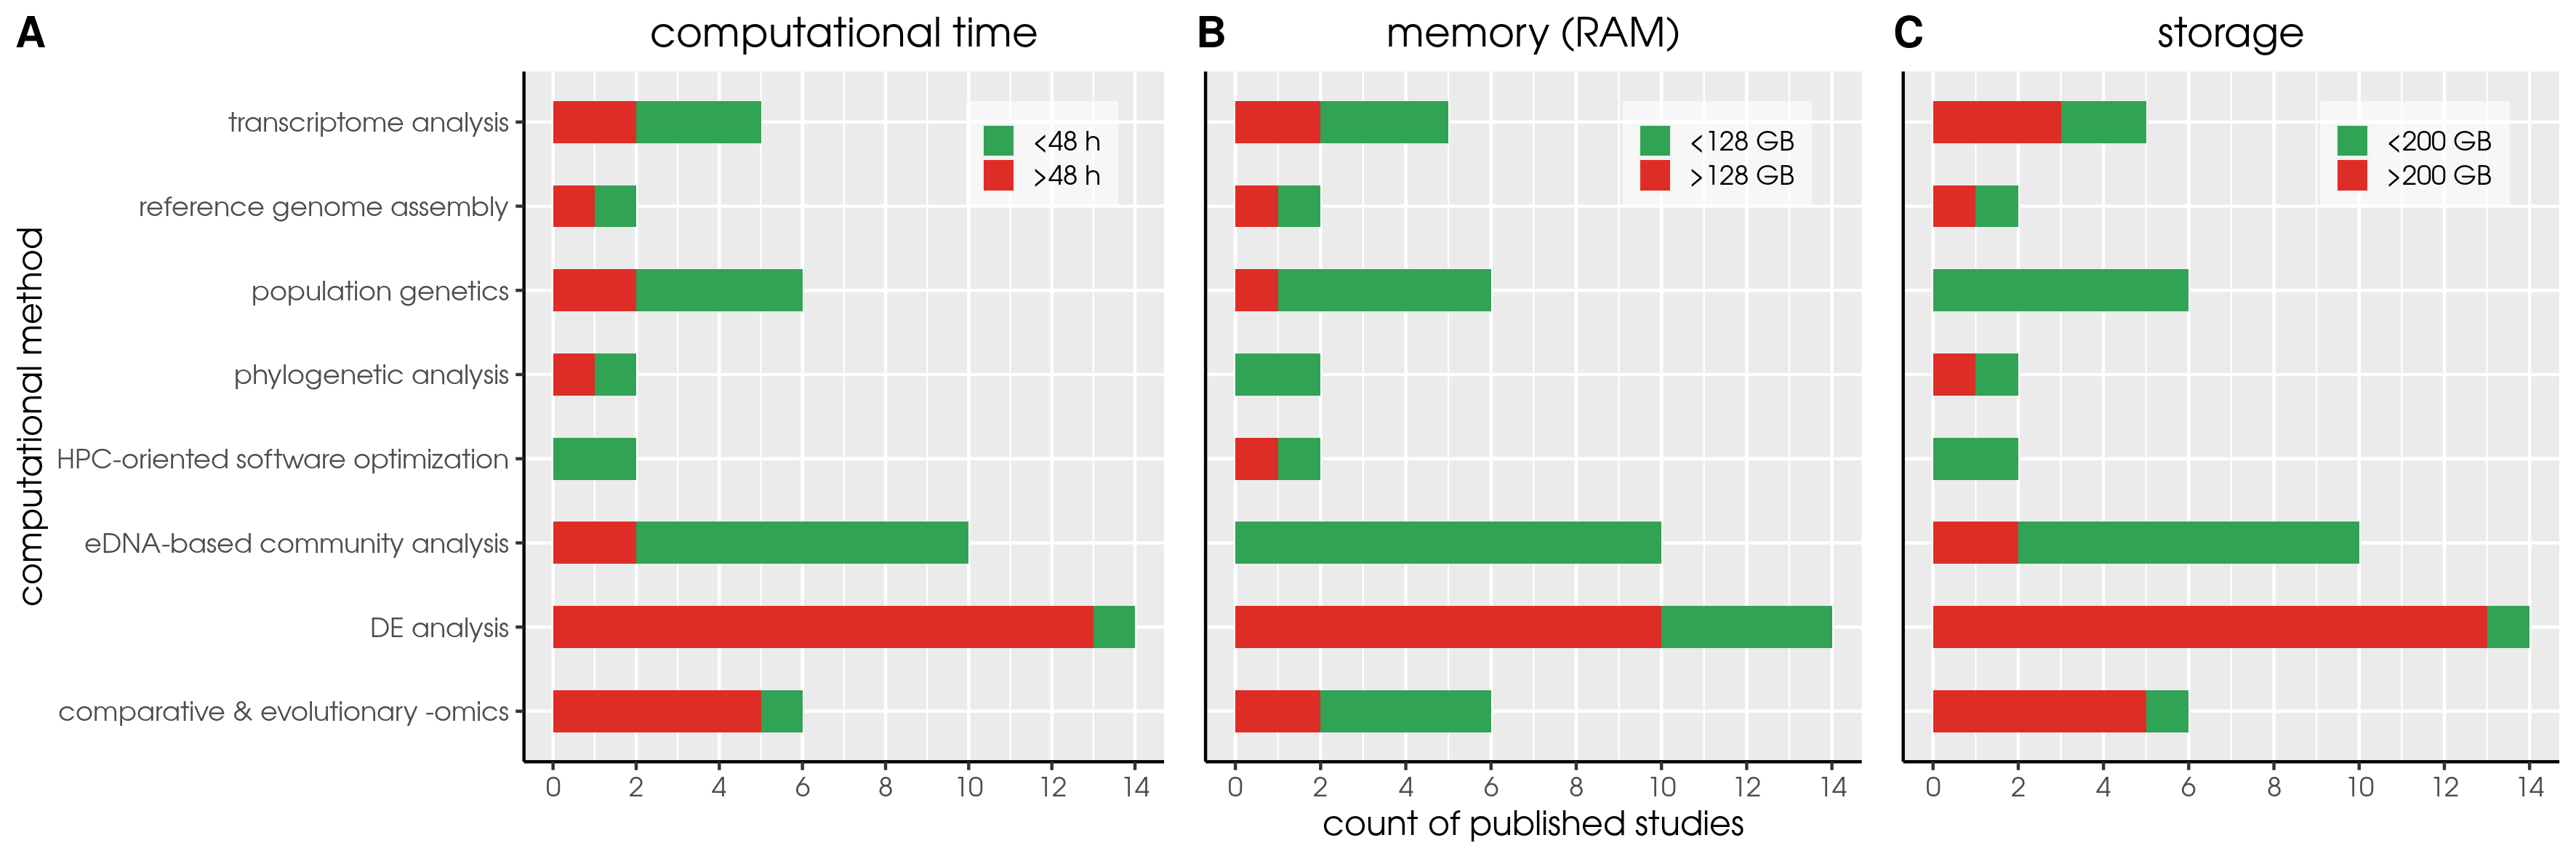
\includegraphics[width=\columnwidth]{figures/computational_method_computational_requirement_plot.png}
      \caption[Computational resources requirements of the so-far published studies supported by the IMBBC HPC facility]{
         Red bars denote published research with high resource requirements of the various computational methods employed at the IMBBC HPC facility due to 
         (a) long computational times ($>48$ h), 
         (b) high memory requirements ($>128$ GB), or 
         (c) high storage requirements ($>200$ GB). 
         For instance, no eDNA-based community analyses performed at \textit{Zorba} thus far have required a large amounts of memory.}
   \end{figure}


   As shown in Fig. 4, the $2$ most commonly used computational methods have rather different resource requirements. 
   While DE analysis shows a notable trend for both long computational times (Fig. 4a) and high memory (Fig. 4b), eDNA-based community analysis does not have high resource requirements either in computation time or memory. 
   High memory was commonly associated with computational methods, including de novo assembly; 
   all relevant research concerned non-model taxa and involved short-read sequencing or combinations of short- and long-read sequencing. 
   By contrast, phylogenetic analysis studies did not involve intensive RAM use; 
   this is largely due to the fact that software used by IMBBC users adopts parallel solutions for tree construction. 
   Long computational times (Fig. 4a) were most often observed at the functional annotation step in transcriptome analysis, DE analysis, and comparative and evolutionary omics, when this step involved BLAST queries of thousands of predicted genes against large databases, such as nr (NCBI). 
   Finally, a common challenge emerging from all bioinformatic approaches is significant storage limitations (Fig. 4c); 
   this challenge was associated with the use of HTS technologies that produce large amounts of raw data, the analysis of which involves the creation of numerous intermediate files.

   Overall, published studies using the IMBBC HPC facility show a degree of variance with respect to the types of tools used 
   (depending on the user, their bioinformatic literacy, and other factors), 
   each of which is more or less optimized with respect to HPC use. 
   Moreover, the variance in computational needs observed within each type of computational method reflects the diversity of the studied taxonomic groups. 
   For instance, transcriptome analysis (involving de novo assembly and functional annotation steps) was employed for the study of taxa as diverse as bacteria, sponges, fungi, fish, and goose barnacles. 
   The complexity of each of these organisms' transcriptomes can, to a large extent, explain the differences observed in computational time, memory, and storage.
   
   Furthermore, \textit{Zorba} CPU and RAM statistics collected since 2019 displayed some overall patterns, including an average computation load per month of less than or close to $50\%$ of its max capacity ($50\%$ of $236$ kilocorehours/month) for most ($20$) of the $24$ months of the logging period. 
   Memory requirements were also heterogeneous: 
   most ($90\%$) of the $44,000$ jobs performed in the same $24$-month period required less than $10$ GB of RAM, and $0.30\%$ of the jobs required more than $128$ GB of RAM 
   (i.e., exceeding the memory capacity of the main compute nodes [\texttt{batch} partition]). 
   The detailed usage statistics of \textit{Zorba} are described in Section B1 and Supplementary file \texttt{zorba\_usage\_statistics.xlsx} of Zafeiropoulos et al. \citep{haris_zafeiropoulos_2021_4665308}.
   
   
   % ZORBA DISCUSSION
   \section{Discussion}

   \subsection{Scientific Impact Stories}

   Below, some examples of research results that were made possible with the IMBBC HPC facility are described. This list of use cases is by no means exhaustive, but rather an attempt to highlight different fields of research supported by the facility, along with their distinct computational features.

   \subsection*{Invasive species range expansion detected with eDNA data from Autonomous Reef Monitoring Structures}

   The Mediterranean biodiversity and ecosystems are experiencing profound transformations owing to Lessepsian migration, international shipping, and aquaculture, which lead to the migration of nearly $1,000$ alien species [46]. 
   The first step towards addressing the effects of these invasions is monitoring of the introduced taxa. 
   A powerful tool in this direction has been eDNA metabarcoding, which has enchanced detection of invasive species \citep{klymus2017environmental}, often preceding macroscopic detection. 
   One such example is the first record of the nudibranch \textit{Anteaeolidiella lurana} (Ev. Marcus \& Er. Marcus, 1967) in Greek waters in 2020 \citep{bariche2020new}. 
   An eDNA metabarcoding analysis allowed for detection of the species with high confidence on fouling communities developed on Autonomous Reef Monitoring Structures (ARMS). 
   This finding, confirmed with image analysis of photographic records on a later deployment period, is an example of work conducted within the framework of the European ASSEMBLE plus programme ARMS-MBON (Marine Biodiversity Observation Network). 
   PEMA software \citep{zafeiropoulos2020pema} was used in this study, as well as in the $30$-month pilot phase of ARMS-MBON \citep{katsanevakis2014invading}.

   \subsection*{Providing omics resources for large genome-size, non-model taxa}

   \textit{Zorba} has been used for building and annotating numerous de novo genome and transcriptome assemblies of marine species, such as the gilthead sea bream \textit{Sparus aurata} \citep{pauletto2018genomic} or the greater amberjack \textit{Seriola dumerili} \citep{sarropoulou2017full}. 
   Both genome and transcriptome assemblies of species with large genomes often exceed the maximum available memory limit, eventually affecting the strategic choices for \textit{Zorba} future upgrades (see Section Future Directions). 
   For instance, building the draft genome assembly of the seagrass Halophila stipulacea (estimated genome size $3.5$ GB) using Illumina short reads has been challenging even for seemingly simple tasks, such as a kmer analysis \citep{tsakogiannis2020importance}. 
   Taking advantage of short- and long-read sequencing technologies to construct high-quality reference genomes, the near-chromosome level genome assembly of Lagocephalus sceleratus (Gmelin, 1789) was recently completed as a case study of high ecological interest due to the species' successful invasion throughout the Eastern Mediterranean \citep{danis2020building}. 
   In the context of this study, an automated containerized pipeline allowing high-quality genome assemblies from Oxford Nanopore and Illumina data was developed (SnakeCube \citep{nelina_angelova_2021_4670966}). 
   The availability of standardized pipelines offers great perspective for in-depth studies of numerous marine species of interest in aquaculture and conservation biology, including rigorous phylogenomic analyses to position each species in the tree of life (e.g., Natsidis et al. \citep{natsidis2019phylogenomics}).

   \subsection*{DE analysis of aquaculture fish species sheds light on critical phenotypes}

   Distinct, observable properties, such as morphology, development, and behavior, characterize living taxa. 
   The corresponding phenotypes may be controlled by the interplay between specific genotypes and the environment. 
   To capture an individual's genotype at a specific time point, molecular tools for transcript quantification have followed the fast development of technologies, with Expressed Sequence Tags as the first approach to be historically used, especially suited for non-model taxa [56]. 
   Nowadays, the physiological state of aquaculture species is retrieved through investigation of stage-specific and immune- and stress response–specific transcriptomic profiles using RNAseq. 
   The corresponding computational workflows involve installing various tools at \textit{Zorba} and implementing a series of steps that often take days to compute. 
   These analyses, besides detecting transcripts at a specific physiological state, have successfully identified regulatory elements, such as microRNAs. 
   Through the construction of a regulatory network with putative target genes, microRNAs have been linked to the transcriptome expression patterns. 
   The most recent example is the identification of microRNAs and their putative target genes involved in ovary maturation \citep{papadaki2020non}.

   \subsection*{Large-scale ecological statistics: are all taxa equal?}

   The nomenclature of living organisms, as well as their descriptions and their classifications under a specific nomenclature code, have been studied for more than $2$ centuries. 
   Up to now, all the species present in an ecosystem have been considered equal in terms of their contributions to diversity. 
   However, this axiom has been tested only once before, on the United Kingdom's marine animal phyla, showing the inconsistency of the traditional Linnaean classification between different major groups \citep{warwick2008all}. 
   In Arvanitidis et al. \citep{arvanitidis2018research}, the average taxonomic distinctness index 
   ($\Delta+$) and its variation ($Lambda+$) were calculated on a matrix deriving from the complete World Register of Marine Species \citep{vandepitte2018decade}, containing more than $250,000$ described species of marine animals. 
   It is the R-vLab web application, along with its HPC high RAM back-end components (on \texttt{bigmem}, see Section The IMBBC HPC Facility: 
   From a Single Server to a Tier 2 System) that made such a calculation possible. This is the first time such a hypothesis has been tested on a global scale. 
   Preliminary results show that the 2 biodiversity indices exhibit complementary patterns and that there is a highly significant yet non-linear relationship between the number of species within a phylum and the average distance through the taxonomic hierarchy.

   \subsection*{Discovery of novel enzymes for bioremediation}

   Polychlorinated biphenyls are complex, recalcitrant pollutants that pose a serious threat to wildlife and human health. 
   The identification of novel enzymes that can degrade such organic pollutants is being intensively studied in the emerging field of bioremediation. 
   In the context of the Horizon 2020 Tools And Strategies to access original bioactive compounds by Cultivating MARine invertebrates and associated symbionts \href{http://www.tascmar.eu/}{(TASCMAR) project}, global ocean sampling provided a large biobank of fungal invertebrate symbionts and, through large-scale screening and bioreactor culturing, a marine-derived fungus able to remove a polychlorinated biphenyl compound was identified for the first time. 
   \textit{Zorba} resources and domain expertise in fungal genomics were used as a Centre for the Study and Sustainable Exploitation of Marine Biological Resources (CMBR) service for the analysis of multi-omic data for this symbiont. Following genome assembly of \textit{Cladosporium sp}. 
   TM-S3 \citep{gioti2020draft}, transcriptome assembly and a phylogenetic analysis revealed the full diversity of the symbiont's multicopper oxidases, enzymes commonly involved in oxidative degradation \citep{nikolaivits2021functional}. 
   Among these, 2 laccase-like proteins shown to remove up to $71\%$ of the polychlorinated biphenyl compound are now being expressed to optimize their use as novel biocatalysts. 
   This step would not have been possible without the annotation of the Cladosporium genome with transcriptome data; 
   mapping of the purified enzymes' LC-MS (Liquid chromatography–mass spectrometry) spectra against the set of predicted proteins allowed for identification of their corresponding sequences.



   \subsection{Lessons Learned}

   \subsection*{Depth and breadth are both required for a bioinformatics-oriented HPC}

   In our experience, the vast majority of the analyses run at the IMBBC HPC infrastructure are CPU-intensive. 
   RAM-intensive jobs ($>128$ GB RAM, see Section Computational Breakdown of the IMBBC HPC-Supported Research) represent only $~0.3\%$ of the total jobs executed over the last $2$ years (see Section B1 in \citep{haris_zafeiropoulos_2021_4665308}). 
   Despite the difference in the frequency of executed jobs with distinct requirements, serving both types of jobs and ensuring their successful completion is equally important for addressing fundamental marine research questions (as shown in Section Computational Breakdown of the IMBBC HPC-Supported Research). 
   The need for both HPC depth (a few high-memory nodes) and breadth (a number of slimmer nodes) has been previously reported \citep{lampa2013lessons}. 
   This need reflects the idiosyncrasy of different bioinformatics analysis steps, often even within the same workflow. 
   High-memory nodes are necessary for tasks such as de novo assembly of large genomes, while the availability of as many less powerful nodes as possible can speed up the execution of less demanding tasks and free resources for other users. 
   Future research directions and the available budget further dictate tailoring of the HPC depth and breadth. Cloud-based services—e.g., for containerized workflows—may also facilitate this process once these become more affordable.

   \subsection*{Quota … overloaded}

   We observed that independently of the type of analysis, storage was an issue for all \textit{Zorba} users (Fig. 4). 
   A high percentage of these issues relate to the raw data from HTS projects. These data are permanently stored in the home directories, occupying significant space. 
   This, in conjunction with the fact that users delete their data with great reluctance, makes storage a major issue of daily use in \textit{Zorba}. 
   In specific cases where users' quota was exceeded uncontrollably, the \textit{Zorba} team has been applying compression of raw and output data in contact with the user, but this is by no means a stable strategy. 
   More generally, with the performance of the existing storage configuration in \textit{Zorba} close to reaching its limits due to the increase in users and its concurrent use, several solutions have been adopted to resolve the issue. 
   The most long-lasting solution has been the adoption of a per user quota system to allow storage sustainability and fairness in our allocation policy. 
   This quota system nevertheless constitutes a limiting factor in pipeline execution, since lots of software tools produce unpredictably too many intermediate files, which not only increase storage but also cause job failures due to space restrictions. 
   We managed the above issue by adding a scratch file system as an intermediate storage area for the runtime capacity needs. 
   Following completion of their analysis, a user retains only the useful files and the rest are permanently removed. 
   A storage upgrade scheduled within 2021 (see Section Future Directions) is expected to alleviate current storage challenges in \textit{Zorba}. 
   However, given the ever-increasing data production (e.g., as the result of decreasing sequencing costs and/or of rising imaging technologies), the responsible storage use approaches described here remain only partial solutions to anticipated future storage needs. 
   Centralized (Tier 1 or higher) storage solutions represent a longer-term solution, which is in line with current views on how to handle big data generated by international research consortia in a long-lasting manner.



   \subsection*{Continuous intercommunication among different disciplines matters}

   Smooth functioning of an HPC system and exploitation of its full potential for research requires stable employment of a core team of computer scientists and engineers, in close collaboration with an extended team of researchers. 
   At least $4$ disciplines are involved in \textit{Zorba}-related issues: 
   computer scientists, engineers, biologists (in the broad sense, including ecologists, genomicists, etc.), and bioinformaticians with varying degrees of literacy in biology and informatics and various domain specializations (comparative genomics, biodiversity informatics, bacterial metagenomics, etc). 
   The continuous communication among representatives of these $4$ disciplines has substantially contributed to research supported by \textit{Zorba} and to the evolution of the HPC system itself over time. 
   In our experience, an HPC system cannot function effectively and for long without full-time system administrators, nor with bioinformaticians alone. 
   Although it has not been the case since the system's onset, investment in monthly meetings, seminars, and training events (in biology, containers, domain-specific applications, and computer science; see Section The IMBBC HPC Facility: From a Single Server to a Tier 2 System) is the only way to establish stable intercommunication among different players of an HPC system. 
   Such proximity translates into timely and adequate systems and bioinformatics analysis support, an element that in its turn translates into successful research (see Section Computational Breakdown of the IMBBC HPC-Supported Research). 
   It should be noted that the overall good experience in connectivity among different HPC players derives from \textit{Zorba} being a Tier 2 system, with a number of active permanent users in double digits. The establishment of such inter-communication was relatively straightforward to implement with periodic meetings and the assistance of ticketing and other management solutions (see Section C1 in \citep{haris_zafeiropoulos_2021_4665308}).


   \subsection*{The way forward: develop locally and share and deploy centrally}
   
   The various approaches regarding the function of an HPC system are strongly related to the different viewpoints of the academic communities towards the relatively new disciplines of bioinformatics and big data. 
   These approaches are strongly affected by national and international decisions that affect the ability to fund supercomputer systems. 
   There are advantages in deploying bioinformatics-oriented HPC systems in centralized (Tier 0 and Tier 1) facilities: 
   better prices at hardware purchases, easier access to HPC-tailored facilities (for instance, in terms of the cooling system and physical space), or experienced technical personnel 
   (see also \citep{lampa2013lessons}). 
   However, synergies between regional (Tier 2) and centralized HPC systems are fundamental for moving forward in supporting the diverse and demanding needs of bioinformatics. 
   An example of such synergies concerns technical solutions (e.g., containerization) that address long-standing software sharing issues. 
   In our experience, a workflow/pipeline can be developed by experts within the context of a specific project in a regional HPC facility. Once a production version of the pipeline is packaged, it can be distributed to centralized systems to cover a broader user audience (see Section The IMBBC HPC Facility From a Single Server to a Tier 2 System). 
   Singularity containers have been developed to utterly suit HPC environments, mostly because they permit root access of the system in all cases. 
   In addition, Singularity is compatible with all Docker images and can be used with Graphics Processing Units (GPUs) and Message Passing Interface (MPI) applications. This is why we chose to run containers in a Singularity format at \textit{Zorba}. 
   However, as Docker containers are widely used, especially in cloud computing (see more about cloud computing in Section Cloud Computing), workflows and services produced at IMBBC are offered in both container formats. 
   Containers are an already established technology, used by the biggest cloud providers worldwide and increasingly by non-profit research institutes. Despite indirect costs (e.g., costs to containerize legacy software), we believe that these technologies will become the norm in the future, especially in the context of reproducibility and interoperability of bioinformatics analysis.


   \subsection*{Software optimizations for parallel execution}

   The most common ways of achieving implicit or explicit parallelization in modern multicore systems for bioinformatics, computational biology, and systems biology software tools are the software threads—provided by programming languages—and/or the OpenMP API \citep{dagum1998openmp}. 
   These types of multiprocessing make good use of the available cores on a multicore system (single node), but they are not capable of combining the available CPU cores from more than 1 node. 
   Some other software tools use MPI to spawn processing chunks to many servers and/or cores or (even better) combine MPI with OpenMP/Threads to maximize the parallelization in hybrid models of concurrency. 
   Such designs are now used to a great extent in some cases, such as phylogeny inference software that makes use of Monte Carlo Markov Chain samplers.
   However, these cases are but a small number compared to the majority of bioinformatics tasks, while their usage in other analyses is low. At the hardware level, simultaneous multithreading is not enabled in the compute nodes of the IMBBC HPC infrastructure. 
   Since the majority of analyses running on the cluster demand dedicated cores, hardware multithreading does not perform well. 
   In our experience, the existence of more (logical) cores in compute nodes misleads the least experienced users into using more threads than the physically available ones, which slows down their executions. 
   In comparison, assisting servers (filesystems, login nodes, web servers) make use of hardware multithreading, since they serve numerous small tasks from different users/sources that commonly contain Input/Output (I/O) operations. 
   GPUs provide an alternative way for parallel execution, but they are supported by a limited number of bioinformatics software tools. Nevertheless, GPUs can optimize the execution process in specific, widely used bioinformatic analyses, such as sequence alignment \citep{vouzis2011gpu, nobile2017graphics}, image processing in microtomography (e.g., microCT), or basecalling of Nanopore raw data.



   \subsection*{Cloud Computing}

   A recent alternative to traditional HPC systems, such as that described in this review, is cloud computing. 
   Cloud computing is the way of organizing computing resources so they are provided over the Internet ("the cloud"). This paradigm of computing requires the minimum management effort possible \citep{mell2011nist}. 
   Cloud computing providers exist in both commercial vendors and academic/publicly funded institutions and infrastructures (for more on cloud computing for bioinformatics, see Langmead and Nellore \citep{langmead2018cloud}). 
   Computing resources can be reserved from individuals, institutions, organizations, or even scientific communities. 
   The most widely-known commercial cloud providers are the “big 3” of cloud computing—namely, 
   \href{https://aws.amazon.com/}{Amazon Web Services}, 
   \href{https://cloud.google.com/}{Google Cloud Platform}, and 
   \href{https://azure.microsoft.com/en-us/}{Microsoft Azure} — while other cloud vendors are constantly emerging. 
   Academic/publicly funded providers are also available: e.g., the \href{https://www.embassycloud.org/}{EMBL–EBI Embassy Cloud}.

   Cloud computing services are being increasingly adopted in research, mainly because they offer simplicity and high availability to users with reduced or even no experience in HPC systems, through web interfaces. 
   For this type of user, the time needed for data manipulation, software installation, and user-system interaction is significantly reduced compared to using a local HPC facility.

   Container technologies, especially Docker, along with container-management systems such as \href{https://kubernetes.io/}{Kubernetes} combined with \href{https://www.openstack.org/}{OpenStack}, have been widely used in a number cloud computing systems, in particular in the research domain. 
   It should be noted, however, that tool experimentation and benchmarking is more limited in cloud computing compared to local facilities and is costly, since it demands additional core hours of segmented computation. 
   In-house HPC infrastructures can be fully configured to suit specific research area needs (storage available, fast interconnection for MPI jobs, number of CPUs versus available RAM, assisting services, etc.). 
   Moreover, in cases where InfiniBand interconnection, a computer networking communications standard, is adopted in HPC, the performance in jobs and software that take advantage of it is substantial. 
   Given the features and advantages of each approach (mentioned above) one could foresee the scenario of combining them to address the research community needs.


   \subsection*{Future Directions}

   An upgrade of the existing hardware design of Zorba has been scheduled in $2021$, funded by the CMBR research infrastructure (Fig. 1). More specifically:

   $3$ nodes of $40$ CPU physical cores will be added through new partitions ($120$ cores in total);
   the total RAM will be increased by $3.5$ TB;
   $100$ TB of cold storage will be installed and is expected to alleviate the archiving problem at the existing homes/scratch file systems; 
   and the total usable existing storage capacity for users in home and scratch partitions will be increased by approximately $100$ TB.
   
   With this upgrade, it is expected that the total computational power of \textit{Zorba} will be increased by approximately $6$ TFlops, while the infrastructure will be capable of serving memory-intensive jobs requiring up to $1.5$ TB of RAM, hosted on a single node. 
   Eventually, more users will be able to concurrently load and analyze big data sets on the file systems. 
   Over the coming $2$ years, \textit{Zorba} is also expected to have $2$ major additions:
   
   \begin{itemize}
      \item  the acquisition of a number of GPU nodes to build a new partition, especially for serving software that has been ported to run on GPUs; and
      \item the design of a parallel file system (Ceph or Lustre) to optimize concurrent I/O operations to speed up CPU-intensive jobs.
   \end{itemize}

   The expectation is that the upcoming upgrade of \textit{Zorba} will further enhance collaborations with external users, since the types of bioinformatic tasks supported by the infrastructure are common to other disciplines beyond marine science, such as environmental omics research in the broad term. 
   A nationwide survey targeting the community of researchers studying the environment and adopting the same approaches (HTS, biodiversity monitoring) has revealed that their computational and training needs are on the rise (A. Gioti et al., unpublished observations). 
   Usage peaks and valleys were observed in \textit{Zorba} (see Section B1 in \citep{haris_zafeiropoulos_2021_4665308}), similarly to other HTS-oriented HPC systems \citep{lampa2013lessons}. 
   It is therefore feasible to share \textit{Zorba}'s idling time with other scientific communities.
   Besides, the \textit{Zorba} upgrade is very timely in coming during a period where additional computational infrastructures emerge: 
   the Cloud infrastructure Hypatia, funded by the Greek node of ELIXIR, is entering its production phase. 
   It will constitute a national Tier 1 HPC facility, designed to host $~50$ computational nodes of different capabilities (regular servers, GPU-enabled servers, Solid-State Drive-enabled servers, etc.) and provide users the option to either create custom virtual machines for their computational services or to upload and execute workflows of containerized scientific software packages. 
   In this context, a strategic combination of \textit{Zorba} and Hypatia is expected to contribute to a strong computational basis in Greece. 
   It is also expected that \textit{Zorba} functionality will be augmented also through its connection with the Super Computing Installations of LifeWatch ERIC (European Research Infrastructure Consortium) (e.g., Picasso facility in Malaga, Spain). 
   Building upon the lessons learned in the last 12 years, a foreseeable challenge for the facility is the enhancement of its usage monitoring to the example of international HPC systems \citep{dahlo2018tracking}, in order to allow even more efficient use of computational resources.



   \section{Conclusions}

   \textit{Zorba} is an established Tier 2 HPC regional facility operating in Crete, Greece. 
   It serves as an interdisciplinary computing hub in the eastern Mediterranean, where studies in marine conservation, invasive species, extreme environments, and aquaculture are of great scientific and socio-economic interest. 
   The facility has supported, since its launch over a decade ago, a number of different fields of marine research, covering all kingdoms of life; 
   it can also share part of its resources to support research beyond the marine sciences.

   The operational structure of \textit{Zorba} enables continuous communication between users and administrators for more effective user support, troubleshooting, and job scheduling. 
   More specifically, training, regular meetings, and containerization of in-house pipelines have proven constructive for all teams, students, and collaborators of IMBBC. 
   This operational structure has evolved over the years based on the needs of the facility’s users and the available resources. 
   The practical solutions adopted—from hardware (e.g., depth/breadth balanced structure, user quotas, and temporary storage) to software (e.g., modularized bioinformatics application maintenance and containerization) and human resource management (e.g., frequent intercommunication, continuous cross-discipline training)—reflect IMBBC research to a large extent. 
   However, and by incrementing previous reviews \citep{lampa2013lessons}, other Institutes and HPC facilities can be informed on the lessons learned (see Section Lessons Learned), and reflect on the computational requirement analysis of the methods presented (see Section Computational Breakdown of the IMBBC HPC-Supported Research) through the spectrum of their own research so as to plan ahead.

   HPC facilities could reach a benefit greater than the sum of their capacities once they interconnect. The IMBBC HPC facility lies at the crossroad of $3$ RIs, CMBR (Greek node of EMBRC-ERIC), LifeWatchGreece (Greek node of LifeWatch ERIC), and ELIXIR Greece, and via these will pursue further collaboration at larger Tier 0 and Tier 1 levels.


